\begin{titlepage}
%
%~\\[1cm]
%régler l'épaisseur des lignes
\newcommand{\HRule}{\rule{\linewidth}{0.5mm}}

\begin{center}
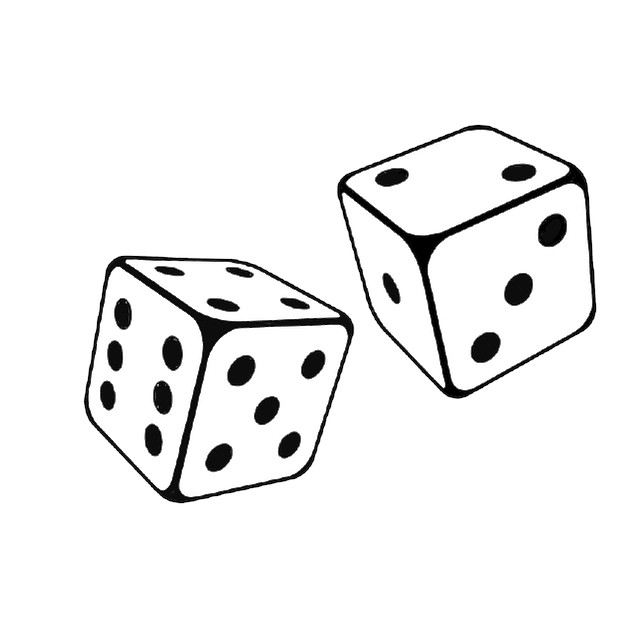
\includegraphics[scale=1.25]{./presentation/deuxDes}
\end{center}

\textsc{\Large }\\[0.5cm]

% Title \\[0.4cm]
\HRule

\begin{center}
{\huge \bfseries  Hasard, déterminisme et\\
philosophie de la contingence\\[0.4cm] }
\end{center}

\HRule \\[1.5cm]


\vfill

\hfill
\begin{minipage}{0.4\textwidth}
\begin{flushright} \large
%\emph{Auteur:}\\
%Stephan \textsc{Runigo}
Extraits de dictionnaires et d'encyclopédies
\end{flushright}
\end{minipage}

\vfill
{\sf \footnotesize
\begin{itemize}[leftmargin=1cm, label=\ding{32}, itemsep=1pt]
\item {\bf Objet : } Étudier les concepts liés au hasard et à la nécessité.
\item {\bf Contenu : } Définitions et philosophie encyclopédique.
\item {\bf Public concerné : } Interressé par la question du hasard.
\end{itemize}
}

\vfill

% Bottom of the page
{\large \today}

\end{titlepage}
